\documentclass{article}

\usepackage{amsmath}
\usepackage[T1]{fontenc}
\usepackage[margin=2.5cm]{geometry}
\usepackage{comment}
\usepackage{graphicx}
\usepackage{float}


\begin{document}
\section{Introduction}
\subsection{The problem of aerodynamic drag}
Dlaczego badamy oraz wzór na opór aerodynamiczny. Że bazujemy na modern exterior balistics i jakieś inne z literatury bo to łądnie brzmi.

\begin{comment}
\subsection{Methodology of the present work}
For simulations we choose two programs to compare the results. The first one is 
Solidworks Flow Simulation, in which we also prepared models for simulations. 
The second one is Ansys Fluent.\\\\
First we prepared the models in Solidworks and from there we exported them to 
.step (214) file format to import them to Ansys. In Ansys we used Fluent with
Meshing to prepare the mesh and then we run the simulations. Solidworks Flow Simulation
was also used to prepare the mesh and run the simulations, which we later compared with
Ansys Fluent results.\\\\
All models were tested using Parametric studies/sets for 9 different velocities 
from 0.1 to 1.0. The resulting graphs of drag coefficient vs mach number were 
compared and analyzed.
\end{comment}

\subsection{Methodology of the present work}
For simulations, two programs were chosen to compare the results. The first program, 
Solidworks Flow Simulation, was used for both CFDs and model preparation. The second 
program utilized was Ansys Fluent.\\\\
Initially, the models were prepared in Solidworks and subsequently exported to 
.step (214) file format for importation into Ansys. Within Ansys, Fluent with 
Meshing was used to prepare the mesh, followed by the execution of simulations. 
Solidworks Flow Simulation was also employed for mesh preparation and simulation execution, 
enabling subsequent comparison with results obtained from Ansys Fluent.\\\\
Parametric studies/sets were conducted for all models, encompassing nine different velocities
ranging from 0.1 to 1.0. Subsequently, resulting graphs depicting the drag coefficient 
versus Mach number were analyzed and compared.



\subsection{Tested models}
R6-Endcone, R6-No-Endcone, PrawieR5\\\\
For each set of simulations, computational domain mesh setting and graph of velocity and 
pressure for 0.6 mach will be shown.\\\\
\newpage
\section{Initial study}
The work was initiated with the remodeled R5 model, which had been prepared in Solidworks 
and featured an endcone, a modification in comparison to the original R5 model. Subsequent 
testing of the model was conducted using Solidworks Flow Simulation. However, this model 
was solely utilized for comparing the results of the older model with the new one. The 
results can be observed here

\begin{figure}[H]
    \centering
    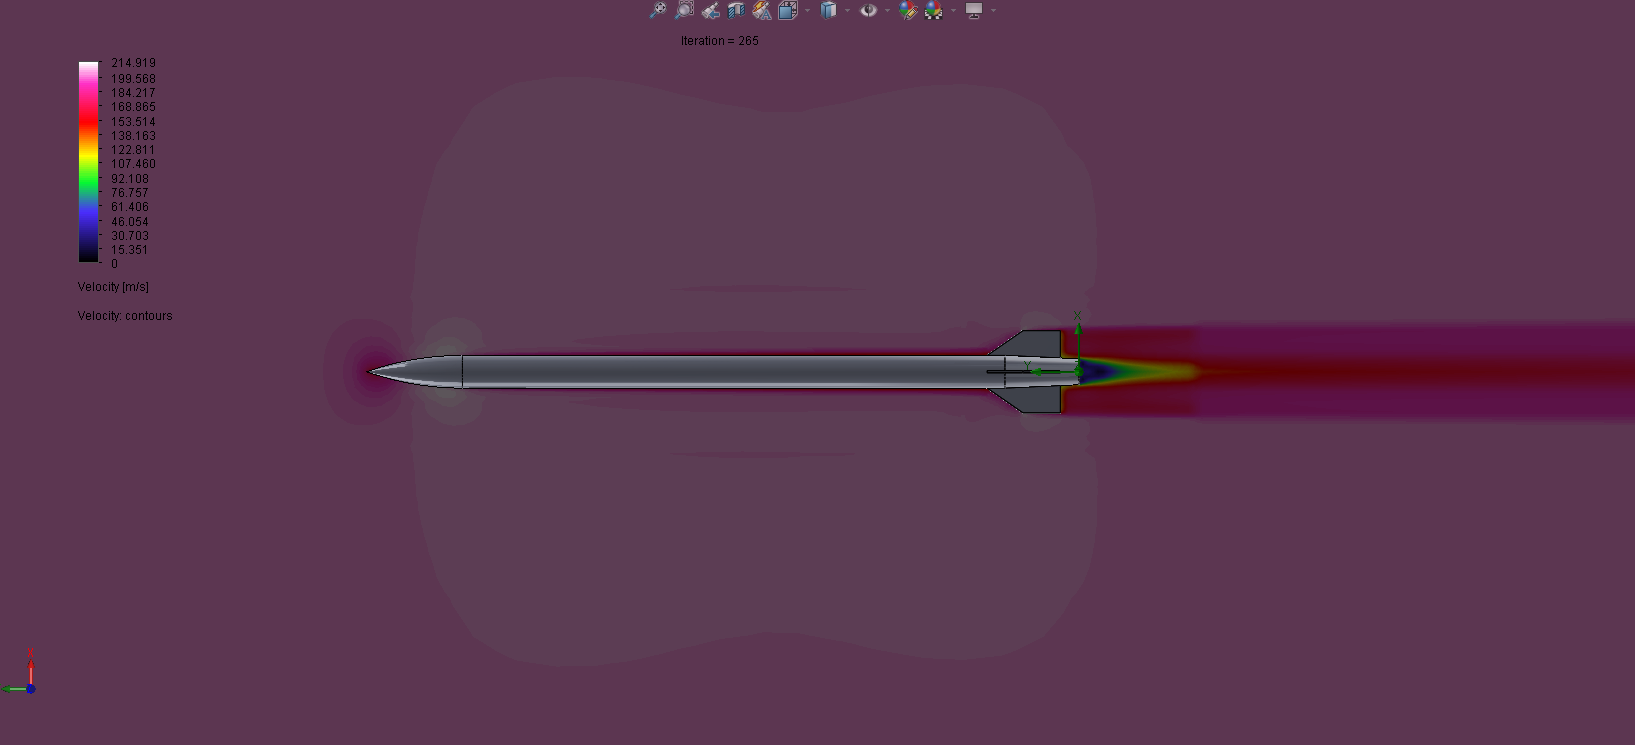
\includegraphics[width=\textwidth]{../data/PrawieR5-Solid/PrawieR5-TR-Velocity-Mach06.png}
    \caption{Velocity graph for PrawieR5 model at Mach 0.6}
\end{figure}

\begin{figure}[H]
    \centering
    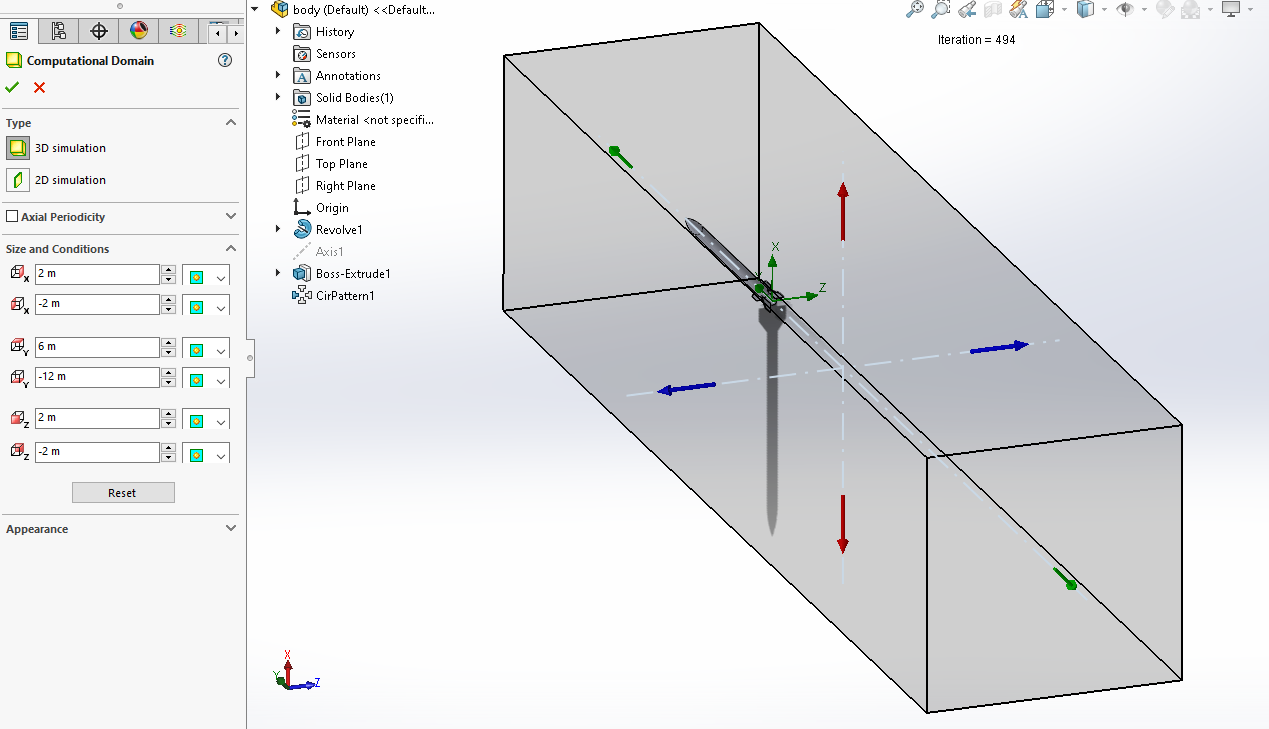
\includegraphics[width=\textwidth]{../data/PrawieR5-Solid/ComputationalDomain.png}
    \caption{CD graph for PrawieR5 model at Mach 0.6}
\end{figure}


\section{Preliminary research of endcone effect in Solidworks}
\subsection{R6 Endcone}
\begin{figure}[H]
    \centering
    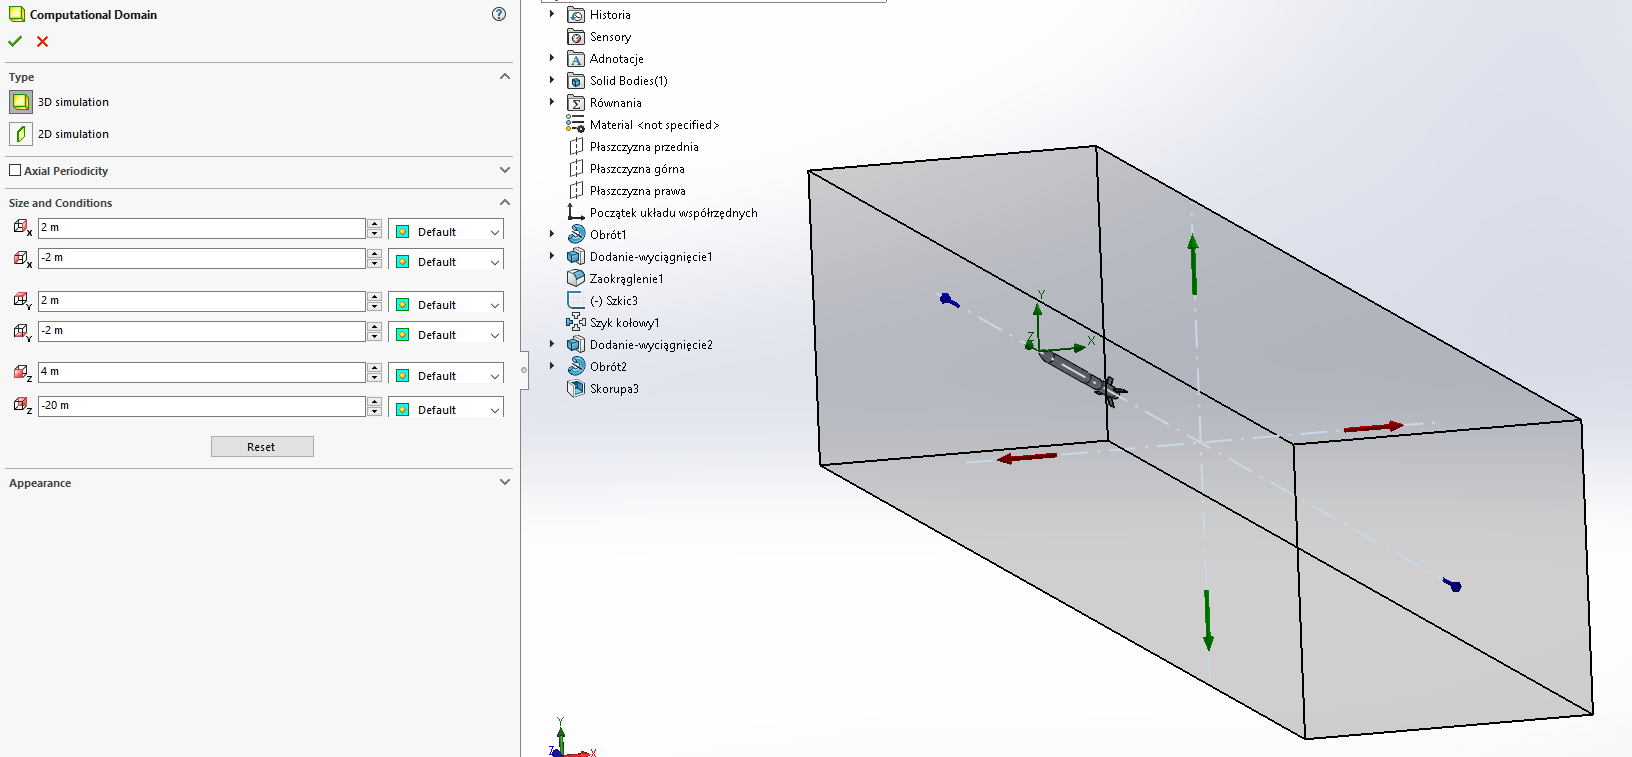
\includegraphics[width=\textwidth]{../data/R6-Endcone-Solid/domain.png}
    \caption{Computational domain for R6-Endcone model}
\end{figure}
\begin{figure}[H]
    \centering
    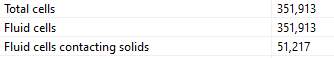
\includegraphics[width=0.6\textwidth]{../data/R6-Endcone-Solid/cells.png}
    \caption{Cell number for R6-Endcone model}
\end{figure}

\begin{figure}[H]
    \centering
    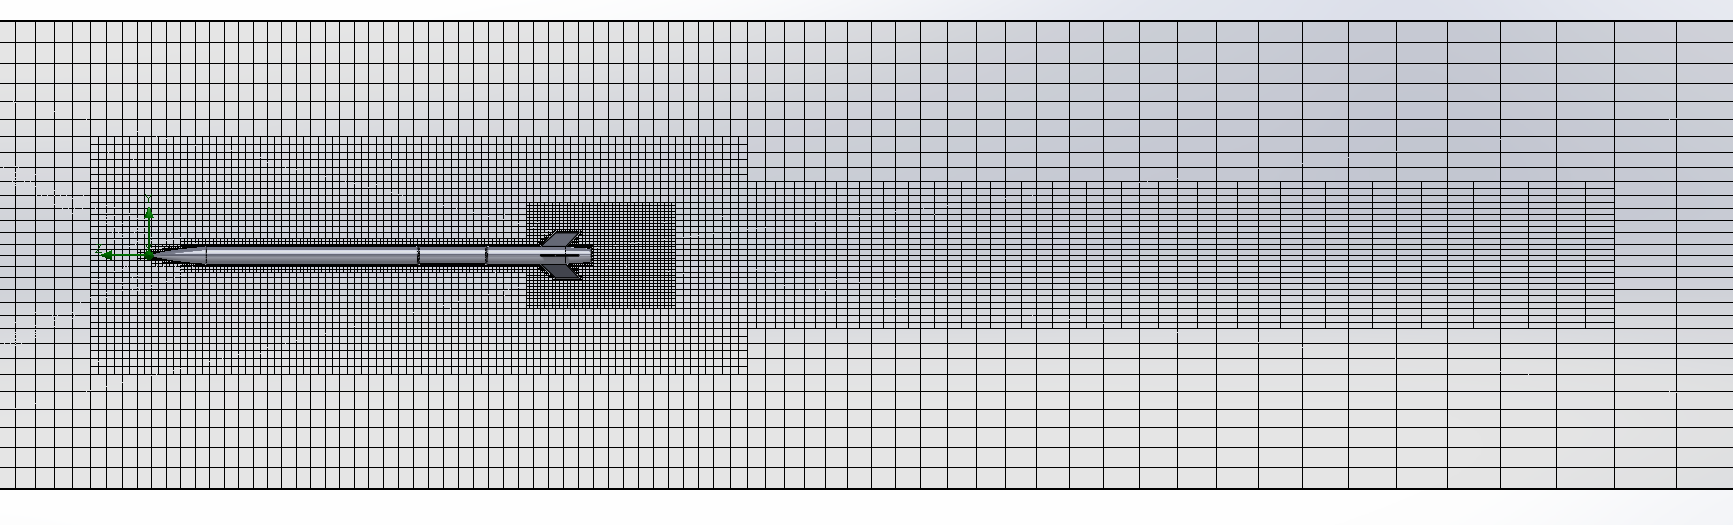
\includegraphics[width=\textwidth]{../data/R6-Endcone-Solid/mesh.png}
    \caption{Mesh for R6-Endcone model}
\end{figure}
\begin{figure}[H]
    \centering
    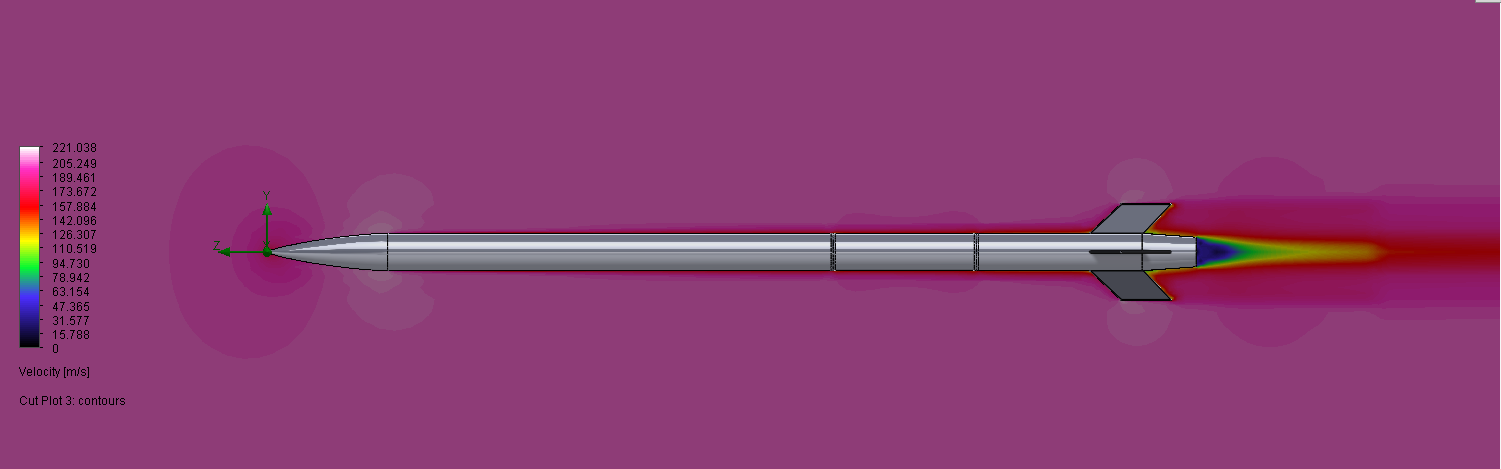
\includegraphics[width=\textwidth]{../data/R6-Endcone-Solid/speed.png}
    \caption{Velocity graph at 0.6 Mach for R6-Endcone model}
\end{figure}

\begin{figure}[H]
    \centering
    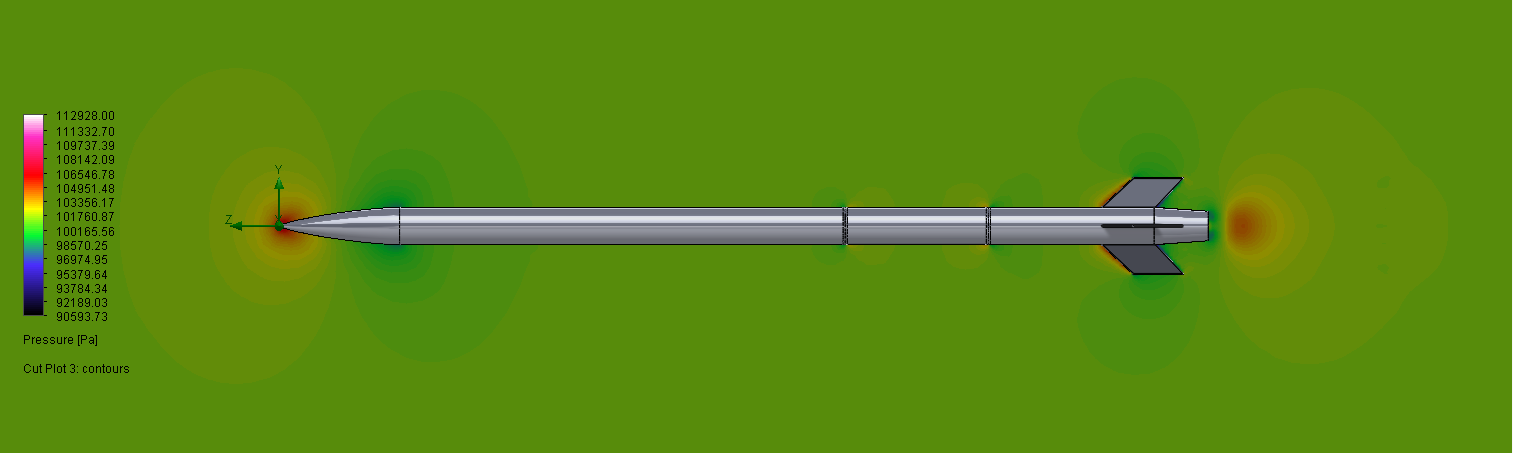
\includegraphics[width=\textwidth]{../data/R6-Endcone-Solid/pressure.png}
    \caption{Pressure graph at 0.6 Mach for R6-Endcone model}
\end{figure}

\subsection{R6 No Endcone}

\begin{figure}[H]
    \centering
    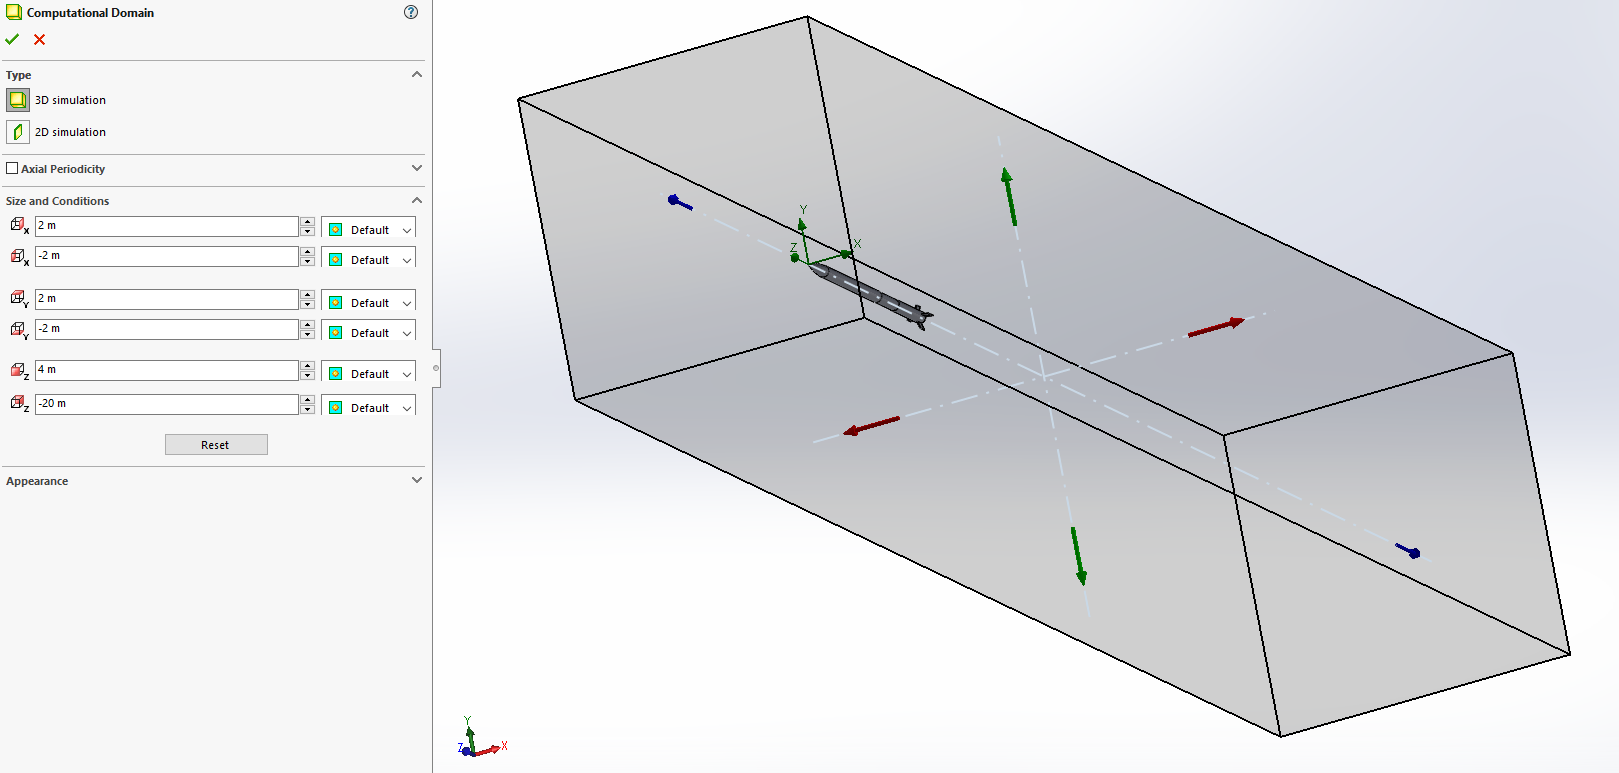
\includegraphics[width=\textwidth]{../data/R6-NoEndcone-Solid/domain.png}
    \caption{Computational domain for R6-NoEndcone model}
\end{figure}
\begin{figure}[H]
    \centering
    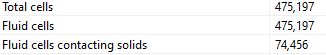
\includegraphics[width=0.6\textwidth]{../data/R6-NoEndcone-Solid/cells.png}
    \caption{Cell number for R6-NoEndcone model}
\end{figure}

\begin{figure}[H]
    \centering
    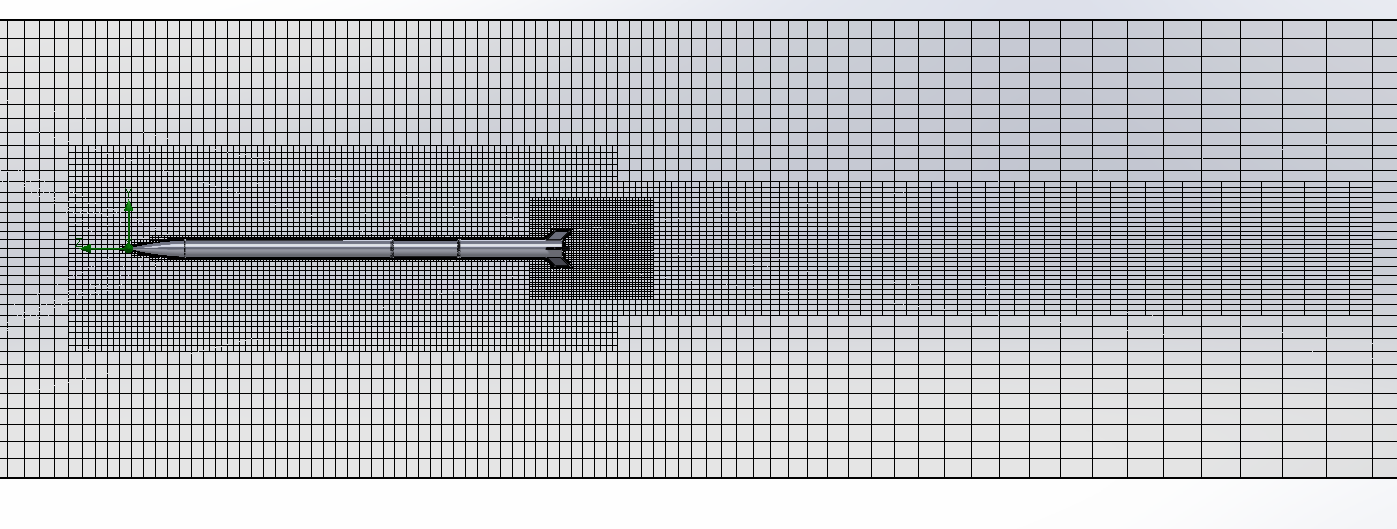
\includegraphics[width=\textwidth]{../data/R6-NoEndcone-Solid/mesh.png}
    \caption{Mesh for R6-NoEndcone model}
\end{figure}
\begin{figure}[H]
    \centering
    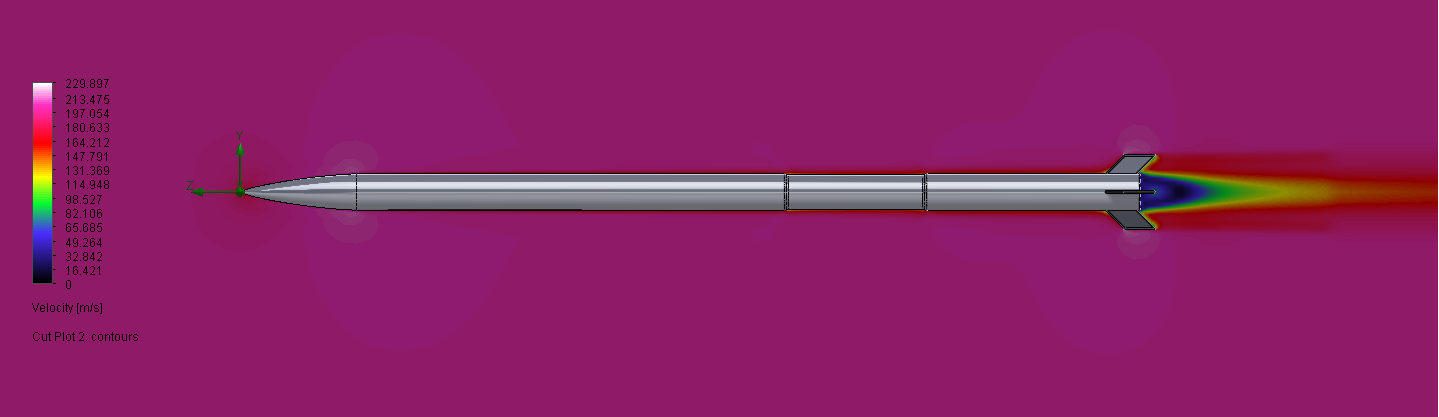
\includegraphics[width=\textwidth]{../data/R6-NoEndcone-Solid/speed.png}
    \caption{Velocity graph at 0.6 Mach for R6-NoEndcone    model}
\end{figure}

\begin{figure}[H]
    \centering
    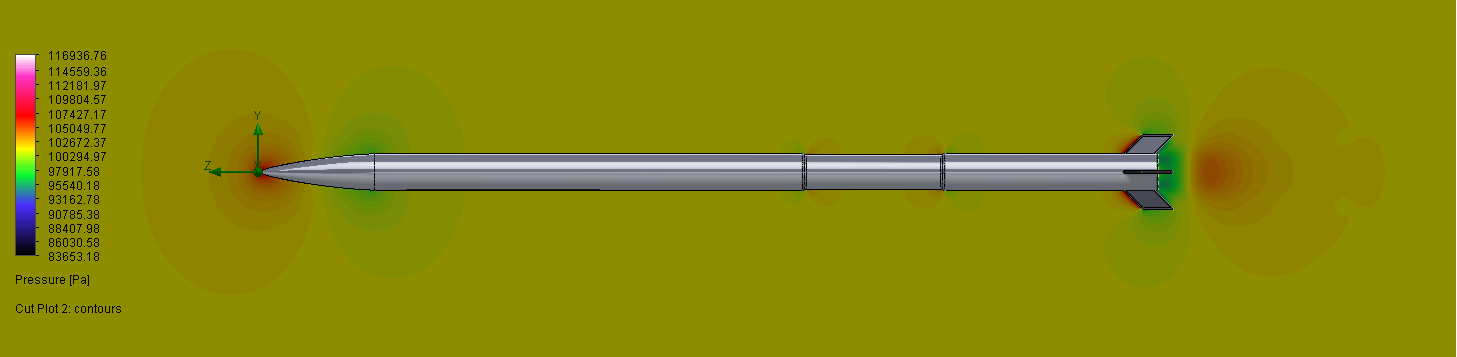
\includegraphics[width=\textwidth]{../data/R6-NoEndcone-Solid/konospeedoatode.png}
    \caption{Pressure graph at 0.6 Mach for R6-NoEndcone model}
\end{figure}

\subsection{Results of the preliminary research}

\begin{figure}[H]
    \centering
    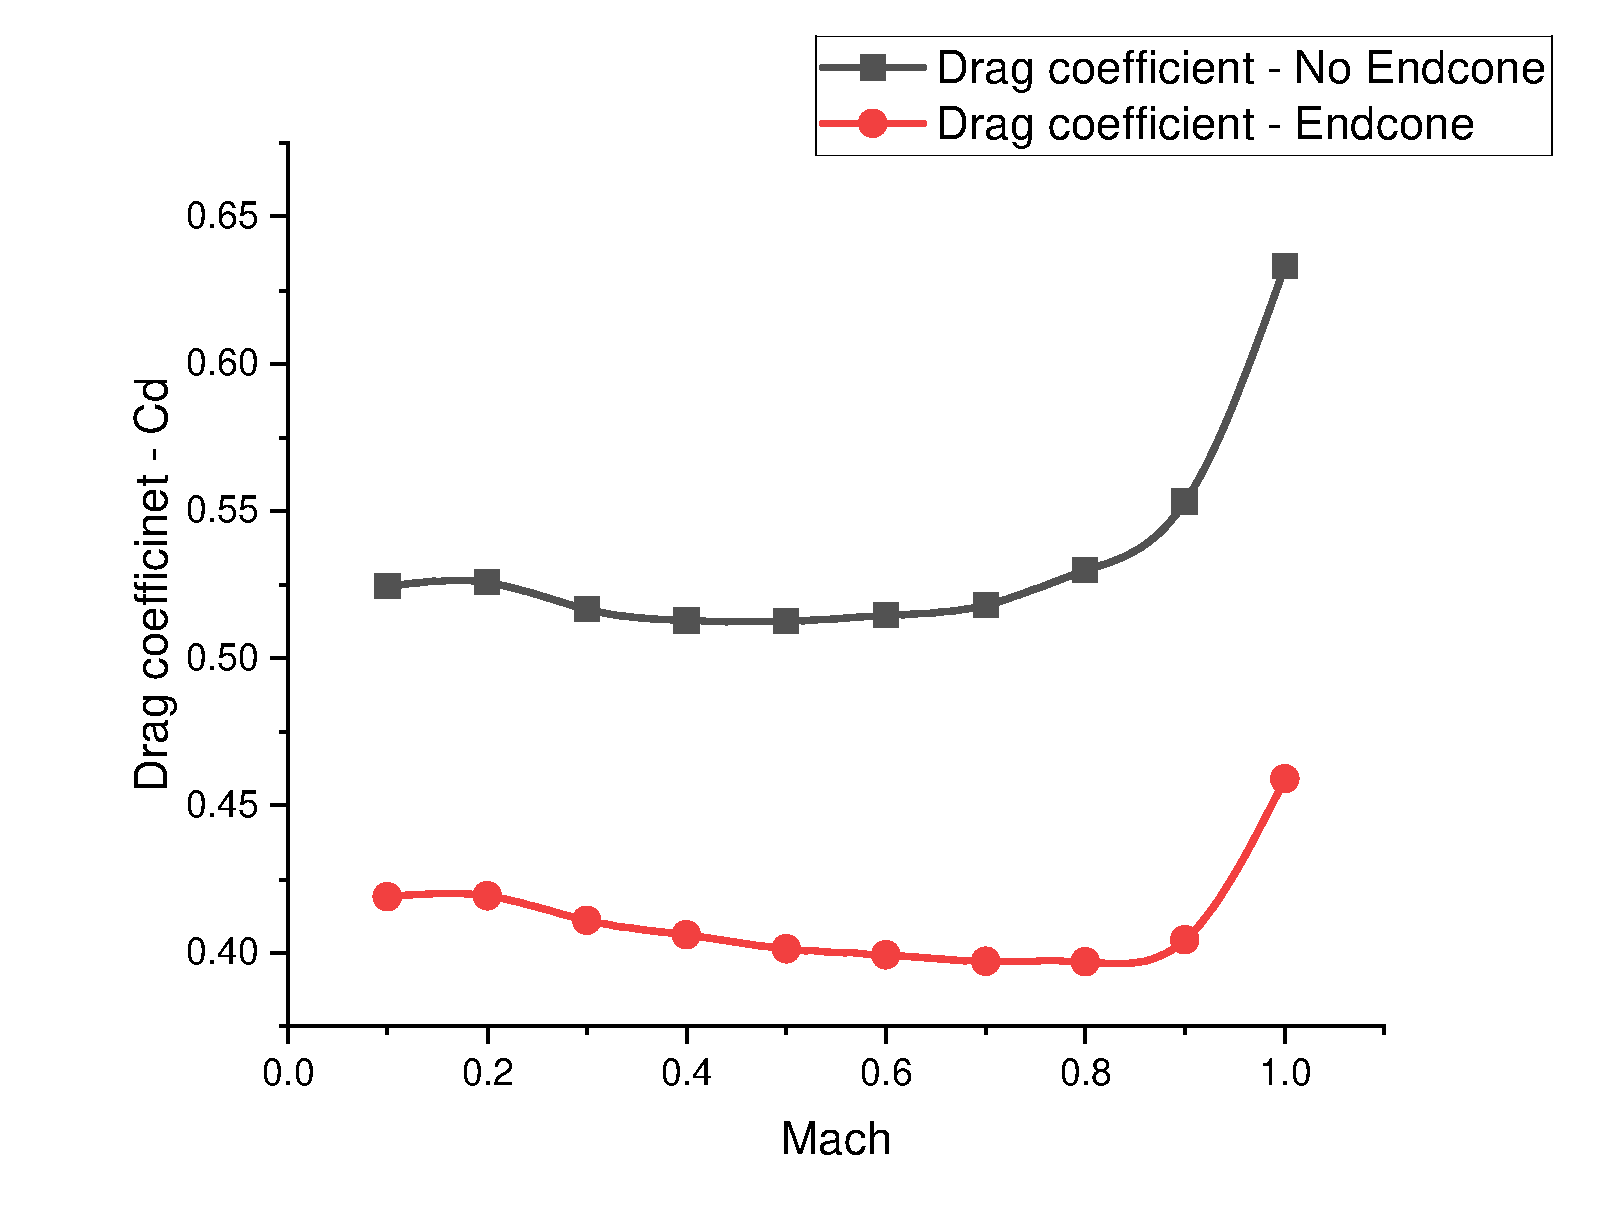
\includegraphics[width=\textwidth]{../data/DataAnalisysSolid/Solid-Studies-CD-Graph.pdf}
    \caption{CD graph of R6-Endcone and R6-NoEndcone models}
\end{figure}
Preliminary research indicates that the endcone model exhibits significantly lower drag coefficient
for 8 degrees endcone angle, while keeping trends of change on the chart. Even more, for endcone model
the trans sonic spike starts later compared to no endcone model. This would be very beneficial for the
range of 0.6-0.9 Mach.  


\begin{table}[H]
    \centering
    \caption{Average values and differences}
    \resizebox{0.8\textwidth}{!}{%
    \begin{tabular}{|c|c|c|c|c|}
        \hline
        & R6 Endcone & R6 No Endcone & Difference & \% Difference \\
        \hline
        0.1 - 1.0 Mach & 0.411 & 0.534 & 0.123 & 29.8\%\\
        \hline
        0.1 - 0.6 Mach & 0.409 & 0.518 & 0.108 & 26.5\%\\
        \hline
    \end{tabular}%
    }
\end{table}
For a range of 0.1 to 0.6 Mach, the endcone model exhibited a 26\% lower drag coefficient in 
comparison to the no endcone model. This is a significant difference, indicating that the endcone
model is much more aerodynamically efficient.

\newpage

\section{Oplitmalization of the endcone in Solidworks}
\subsection{Range and goal of this study}
The goal of this study was to find a minimum of the average drag force function, depending on
the endcone angle, which was coupled to the lenght of the endcone. The range of the
study was from 3 to 15 degrees, with a step of 1 degree. For each angle, simulations were preformed for 
0.1 to 0.6 Mach, with a step of 0.1 Mach. In total 96 simulations were made, however it since 
lenghts of encone for angle values of 0 - 3 were too big, those where deleted from study.\\\\
Finding minimum of the average drag force function is crucial for the optimalization of the rocket
since that would allow to reduce the drag force acting on the rocket, which would result in
overall better performance of the rocket.\\\\
Function of drag coefficient for different Mach number depending on the endcone angle is also 
shown in the graph. It allows to determine the optimal angle for the endcone for specific
velocity and can be compared with existing literature.\\\\
Mesh and domain settings for following simulations are the same as in the preliminary research for
R6-Endcone model. Cell count changed slightly with the change of the endcone angle, but it was
negligible.

\subsection{Results and discussion}

\begin{figure}[H]
    \centering
    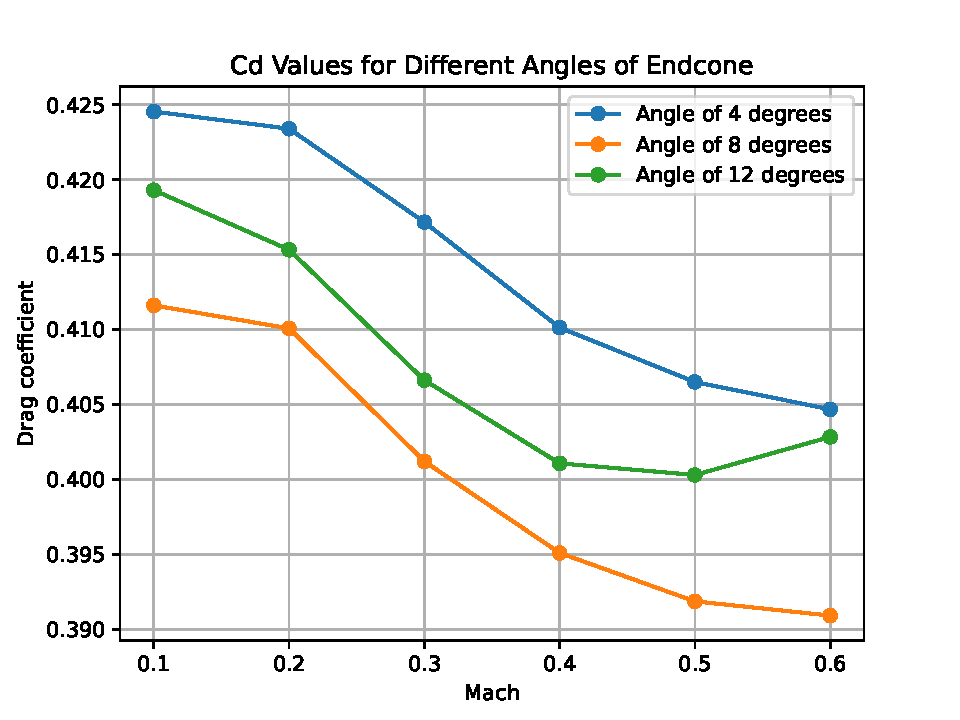
\includegraphics[width=\textwidth]{../data/R6-Parametric-Endcone/ExampleCdGraphs.pdf}
    \caption{Example of CD graphs for different endcone angles}
\end{figure}

\begin{figure}[H]
    \centering
    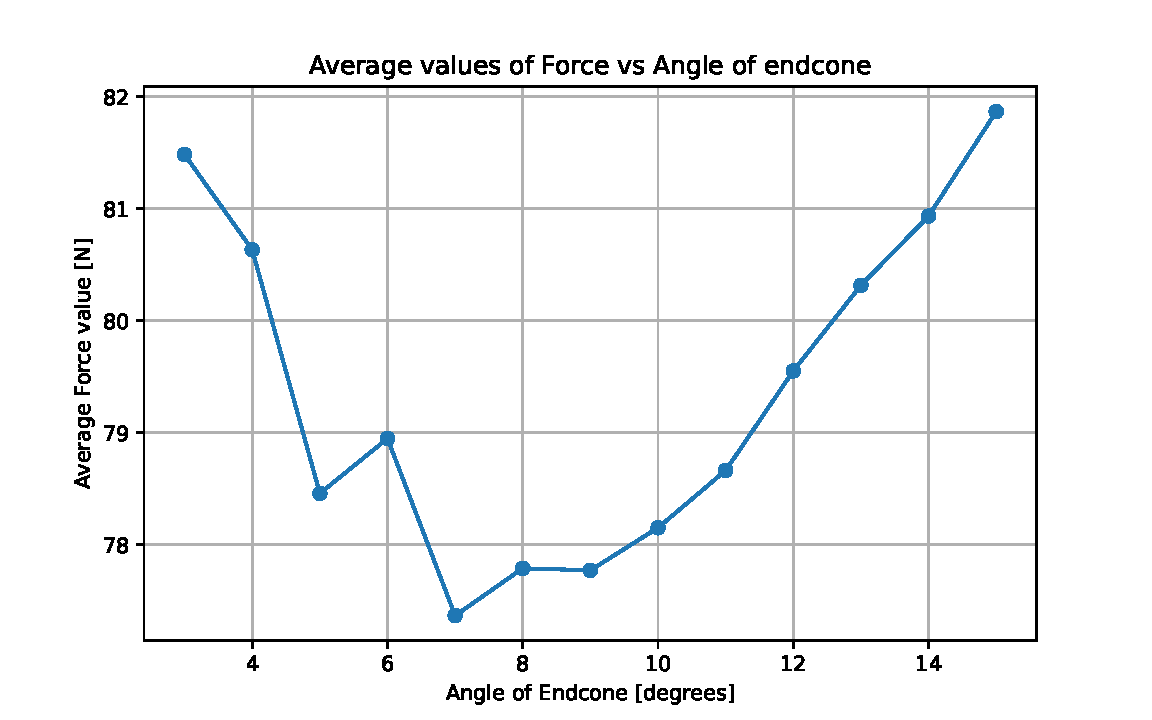
\includegraphics[width=0.8\textwidth]{../data/R6-Parametric-Endcone/ForceVsAngle.pdf}
    \caption{Average Force vs Angle graph}
\end{figure}
As we can see, the minimum of the average drag force function is at 7 - 9 degrees. We can also 
observe a trend of the function, which is decreasing for the range of 3 to 7 degrees and increasing
for the range of 9 to 15 degrees.\\\\
Spike at 6 degree is also worth mentioning, it may be true value at this point or just a result of
the simulation error. This would require further research to determine the validity of this spike, however 
it is not crucial for the optimalization of the rocket, since it is much higher than the minimum 
of the function and it's unlikely that noise of simulation was that high.

\begin{figure}[H]
    \centering
    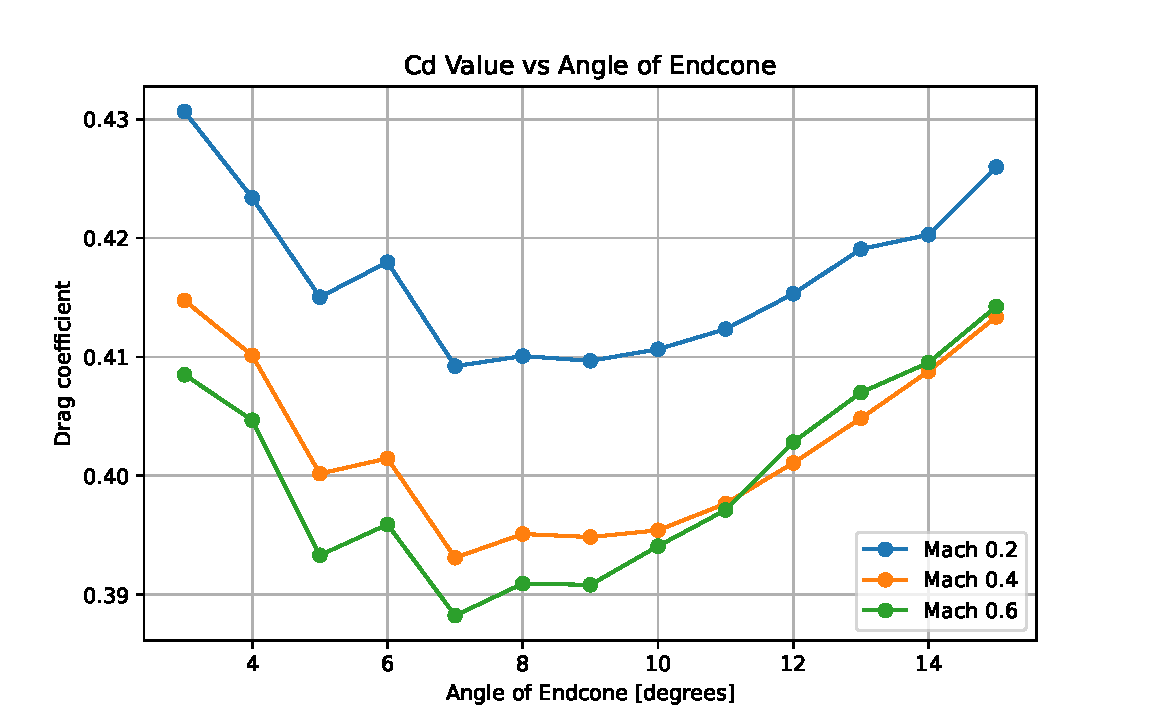
\includegraphics[width=0.8\textwidth]{../data/R6-Parametric-Endcone/CdVsAngle.pdf}
    \caption{Drag coefficient vs Angle graph}
\end{figure}

\newpage

\section{Optimalization of the endcone in Ansys Fluent}
\begin{enumerate}
    \item What we did - optimalization depending on angle - 0.1 - 0.6 Mach and 1 or 2 degree step for some range.
    \item Stability changes depending on angle - Graph from OpenRocket
    \item Domain and Mesh, Speed and Pressure graphs for 0.6 Mach
    \item Results and discussion - mention that endcone is 4 degrees because of manufacture.
\end{enumerate}

\section{Optimalization fin sweep angle in Ansys Fluent}
\begin{enumerate}
    \item What we did - optimalization depending on angle - 0.1 - 0.6 Mach and 1 or 2 degree step for some range. 
    This all for 4 degree endcone angle.
    \item Stability changes depending on angle - Graph from OpenRocket
    \item Domain and Mesh, Speed and Pressure graphs for 0.6 Mach - BEST SAME AS BEFORE
    \item Results and discussion, mention that the final results can be 
\end{enumerate}

\section{Summary and discussion}
Results were great success, unlukcy with endcone being 4 degrees, but still great.

\end{document}